% \iffalse meta-comment
%
% Copyright (C) 2017 Roland Hieber <rohieb+latex-zube-Ua2thei6@rohieb.name>
% -------------------------------------------------------------------------
% 
% This file may be distributed and/or modified under the
% conditions of the LaTeX Project Public License, either version 1.3
% of this license or (at your option) any later version.
% The latest version of this license is in:
%
%    http://www.latex-project.org/lppl.txt
%
% and version 1.3 or later is part of all distributions of LaTeX 
% version 2005/12/01 or later.
%
% This work has the LPPL maintenance status `maintained', and the Current
% Maintainer of this work is Roland Hieber.
%
% This work consists of the files `zube.dtx` and `zube.ins`, as well as the
% derived files `zube.sty` and `zube.pdf`.
%
% \fi
%
% \iffalse
%<*driver>
\ProvidesFile{zube.dtx}
%</driver>
%<package>\NeedsTeXFormat{LaTeX2e}[2005/12/01]
%<package>\ProvidesPackage{zube}
[2017/07/20 v1.0 Zuwendungsbestätigung nach Par. 10 EStG]
%
%<*driver>
\documentclass{scrdoc}
\usepackage{zube}[2017/07/20]
\usepackage[utf8]{inputenc}
\usepackage[ngerman]{babel}
\EnableCrossrefs
\CodelineIndex
\RecordChanges
\begin{document}
  \DocInput{zube.dtx}
\end{document}
%</driver>
% \fi
%
% \CheckSum{0}
%
% \changes{v1.0}{2017/07/20}{Initiale Version}
%
% \GetFileInfo{zube.dtx}
%
% \DoNotIndex{\newcommand,\newenvironment}
% 
%
% \title{Das Paket \textsf{zube}\thanks{Dieses Dokument entspricht
%   \textsf{zube}~\fileversion  mit Datum \filedate.}}
% \author{Roland Hieber\\ \texttt{rohieb+latex-zube-Ua2thei6@rohieb.name}}
%
% \maketitle
%
% \section{Einleitung}
%
% Jede gemeinnützige, steuerbegünstigte Einrichtung erhält irgendwann einmal
% Spenden, sei es in Form von Geldzuwendungen oder Sachspenden. Sofern dies nur
% gelegentlich passiert, können die entsprechenden Formulare für die Bestätigung
% der Zuwendung an den Spender noch händisch ausgefüllt und verschickt werden.
% Mit steigendem Spendenaufkommen ist es allerdings ratsam, den Prozess des
% Ausfüllens zu automatisieren. Dazu soll dieses \LaTeX{}-Paket dienen.
%
% Dieses Paket benutzt dabei die originalen Formulare der Bundesfinanzverwaltung
% Finanzen der Bundesrepublik Deutschland.
%
% \section{Benutzung}
%
% TODO
%
% \StopEventually{\PrintChanges\PrintIndex}
%
% \section{Implementierung}
%
%    \begin{macrocode}
\RequirePackage{geometry}[2010/09/12]
\RequirePackage{graphicx}
\RequirePackage{pdfpages}
\RequirePackage[absolute]{textpos}
\RequirePackage{xcolor}

\RequirePackage{xkeyval}
\define@cmdkeys{zube}[zube@]{
	aussteller,
	ausstellerLogo,
	zuwendender,
	betragInZiffern,
	betragInBuchstaben,
	datumZuwendung,
	beguenstigteZwecke,
	finanzamt,
	stNr,
	unterschriftOrt,
	unterschriftDatum,
	unterschriftNameA,
	unterschriftNameB,
}
\define@boolkeys{zube}[zube@]{
	verzichtVonAufwendungen,
	befreiungKStGewSt,
	feststellungAO,
	mitgliedsbeitragAbziehbar,
	showboxes,
}{}
% Abschnitt Befreiung von Körperschafts- und Gewerbesteuer
\define@cmdkeys{zube}[zube@]{bkgBeguenstigteZwecke  }[\zube@beguenstigteZwecke]
\define@cmdkeys{zube}[zube@]{bkgFinanzamt           }[\zube@finanzamt]
\define@cmdkeys{zube}[zube@]{bkgStNr                }[\zube@stNr]
\define@cmdkeys{zube}[zube@]{bkgDatum               }
\define@cmdkeys{zube}[zube@]{bkgVeranlagungszeitraum}

% Abschnitt Feststellung der satzungsmäßigen Voraussetzungen nach § 60a AO
\define@cmdkeys{zube}[zube@]{faoBeguenstigteZwecke  }[\zube@beguenstigteZwecke]
\define@cmdkeys{zube}[zube@]{faoFinanzamt,          }[\zube@finanzamt]
\define@cmdkeys{zube}[zube@]{faoStNr,               }[\zube@stNr]
\define@cmdkeys{zube}[zube@]{faoDatum,              }

\newcommand{\zube@selectfont}{\fontsize{10pt}{11pt}\itshape\selectfont}

\newcommand{\zubeBoxCheckmark}{{\fontsize{18pt}{18pt}\selectfont\upshape X}}

\newcommand{\zubeGeldVerein}[3]{
	%\presetkeys{zube}{
		%verzichtVonAufwendungen=false,
		%unterschrift
	%}{}
	\setkeys{zube}{aussteller={#1}}
	\setkeys{zube}{zuwendender={#2}}
	\setkeys{zube}{#3}
	%\presetkeys{zube}{
		%verzichtVonAufwendungen=false,
		%unterschriftNameA={},
		%unterschriftNameB={},
		%faoFinanzamt=\usevalue{finanzamt},
		%bkgFinanzamt=\usevalue{finanzamt},
	%}{}

	{ % push font stack

	\cleardoublepage
	\thispagestyle{empty}
	\TPoptions{absolute=true}
	\TPoptions{absolute=true,showboxes=\ifzube@showboxes true\else false\fi}
	\textblockrulecolour{red}
	\textblockorigin{1mm}{1mm}
	\setlength{\TPHorizModule}{1mm}
	\setlength{\TPVertModule}{\TPHorizModule}
	
	\begin{textblock}{1}(0,0)
		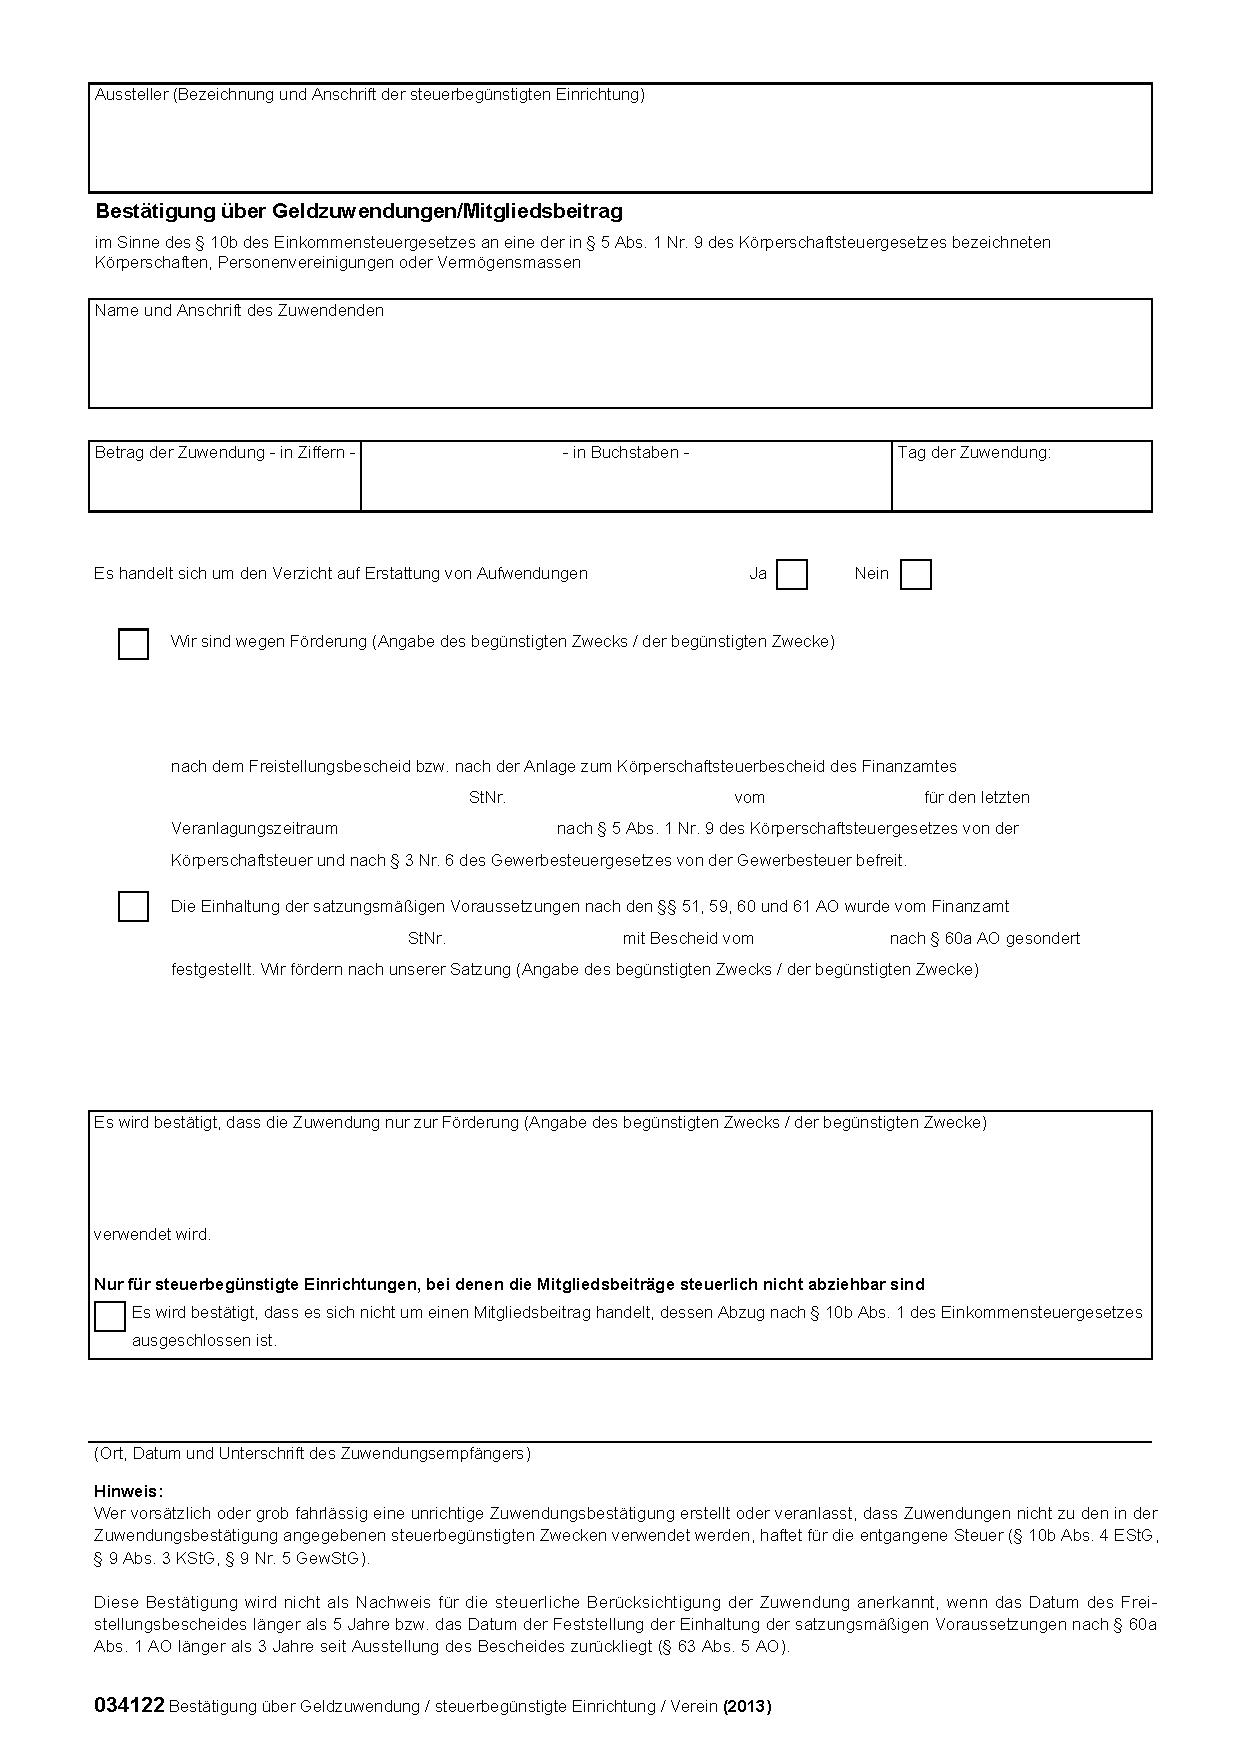
\includepdf[pages=1]{form034122.pdf}
	\end{textblock}
	\newlength{\zube@saveindent}
	\setlength{\zube@saveindent}{\parindent}
	\setlength{\parindent}{0pt}
	
	\zube@selectfont
	
	\begin{textblock}{174}(17,18)
		\zube@aussteller
	\end{textblock}

	\begin{textblock}{174}(17,55)
		\zube@zuwendender
	\end{textblock}

	\begin{textblock}{38}(17,80)
		\centering \zube@betragInZiffern
	\end{textblock}
	\begin{textblock}{83}(64,80)
		\centering \zube@betragInBuchstaben
	\end{textblock}
	\begin{textblock}{38}(154,80)
		\centering \zube@datumZuwendung
	\end{textblock}

	\ifzube@verzichtVonAufwendungen
		\begin{textblock}{4}(131.12,94)
			\centering \zubeBoxCheckmark
		\end{textblock}
	\else
		\begin{textblock}{4}(152.12,94)
			\centering \zubeBoxCheckmark
		\end{textblock}
	\fi

	\ifzube@befreiungKStGewSt
		\begin{textblock}{4}(19.6,105.8)
			\centering \zubeBoxCheckmark
		\end{textblock}
		\begin{textblock}{155}(28,111)
			\zube@bkgBeguenstigteZwecke
		\end{textblock}
		\begin{textblock}{47}(28,132.4)
			\zube@bkgFinanzamt
		\end{textblock}
		\begin{textblock}{36}(86,132.4)
			\centering \zube@bkgStNr
		\end{textblock}
		\begin{textblock}{24}(130,132.4)
			\centering \zube@bkgDatum
		\end{textblock}
		\begin{textblock}{33}(58,137.8)
			\centering \zube@bkgVeranlagungszeitraum
		\end{textblock}
	\fi

	\ifzube@feststellungAO
		\begin{textblock}{4}(19.6,150.2)
			\centering \zubeBoxCheckmark
		\end{textblock}
		\begin{textblock}{39}(28,156.2)
			\zube@faoFinanzamt
		\end{textblock}
		\begin{textblock}{27}(76,156.2)
			\centering \zube@faoStNr
		\end{textblock}
		\begin{textblock}{21}(128,156.2)
			\centering \zube@faoDatum
		\end{textblock}
		\begin{textblock}{155}(28,167)
			\zube@faoBeguenstigteZwecke
		\end{textblock}
	\fi

	\begin{textblock}{170}(17,194)
		\zube@beguenstigteZwecke
	\end{textblock}

	\ifzube@mitgliedsbeitragAbziehbar
		\begin{textblock}{4}(15.6,219.6)
			\centering \zubeBoxCheckmark
		\end{textblock}
	\fi

	\begin{textblock}{70}(15,239)
		\zube@unterschriftOrt, \zube@unterschriftDatum
	\end{textblock}
	\begin{textblock}{50}(91,244)
		\centering \zube@unterschriftNameA
	\end{textblock}
	\begin{textblock}{50}(144,244)
		\centering \zube@unterschriftNameB
	\end{textblock}

	} % pop font stack

	% cleanup
	\setlength{\parindent}{\zube@saveindent}
	\phantom{some content to get cleardoublepage to work}
	\cleardoublepage
}
%    \end{macrocode}
% \Finale
\endinput
% vim: ft=tex ts=2 sw=0 noet tw=80 indentexpr=
